%!TEX root = ../dissertation.tex
\begin{savequote}
We don't want to focus on the trees (or their leaves) at the expense of the forest.
\qauthor{Douglas R. Hofstadter}
\end{savequote}

\chapter{The Brain}
\label{cap:thebrain}

The sensory apparatus of single cell organisms is directly linked to their motor apparatus, meaning that structures capable of detecting perturbations are tightly coupled to structures capable of generating movement \cite[p.~149]{maturana1987tree}. In protozoa, for example, the same flagellum that moves it in the environment also detects obstacles, while some bacteria have chemotaxing mechanisms that change direction of movement, increasing or reducing tumbling rate, in direct response to changes in sugar concentration \cite[p.~147-149]{maturana1987tree}. The coupling between sensory and motor surfaces (i.e. what to do in response to perceived environment), in these direct links, is inflexible.

In contrast to direct sensory-motor connections, the nervous system appears as an intermediate component between the surfaces of interaction of an organism with the surrounding environment. A nervous system endows its owner with structural plasticity, thus enabling learning via changes in this intermediate step between sensory and motor surfaces, producing bigger behavioral repertoires and complex behavior \cite[p.~175]{maturana1987tree}. This comes at the expense of a lot of energy: up to 20\% of human total resting metabolism \cite{attwell2001energy}, which is used mainly by \textit{neurons} \cite{zhu2012quantitative}, a cell type that receives, modulates, and sends signals. The reason why so much of our energy budget is directed towards this single type of cell, can possibly be explained by the importance of its activity for the organism.

With the intermediate system increasing in size, the motor output gets farther apart from the sensory input. The motor output, or behavior, is still conditioned in the organism's perception of the environment, but now abstractions away from the sensory apparatus. On the one hand, some environment characteristics such as a predator's smell or presence of a hurtful shock may have direct impact on behavior. Other ones, such as the identity of objects or the passage of time, may need to be abstracted from the raw sensory input. The specific way in which nervous systems, and in special the brain, produce or develop representations of these environment characteristics to guide behavior, is a central question since the creation of neuroscience.

\textcolor{red}{Here we are missing a paragraph. Why did you say all these things above. You may want to say that they were your inspiration for the study, for getting in neuroscience? The statements above are fairly genneral, so you need a connection to what you are going to say next... }

The introduction was divided into three chapters. In this first, we gave a high-level view of some of the neuroscience challenges and techniques to tackle them, along with the framework that encompasses the rest of the dissertation. In chapter \ref{chap:timing} we characterize the field of \textit{timing}, that encircles and motivates our questions. At last, in chapter \ref{chap:where} we close into our specific motivations and objectives.

\section{What the brain really does}
\label{sec:theory}
    We know that the nervous system mediates the interaction between a living system's sensory inputs, i.e., what is perceived from the environment, and the system's output, e.g., movement. Based only on excitatory and inhibitory connections between neurons, even in the simplest unidirectional case, it is possible to generate reasonably complex behaviors, which can be interpreted as fear responses, aggression, or even logic \cite{braitenberg1986vehicles}. % Possivelmente uma imagem do vehicles, tipo figura 5 pg13
    
    In extremely simple circuits, such as the ones described above, it may be possible to generate mechanistic accounts of this mediation, providing an effective explanation to phenomena like reflex arcs. With little complexity added, these explanations can get really intricate, as in the case of the much-studied Somatogastric Ganglion (STG) of the lobster. The gastric circuit within the STG generates complex oscillatory patterns with a circuit of only 11 neurons \cite{selverston2009neural}. Despite this circuit's smallness, it took 30 years from their discovery to the development of mechanistic explanations for its functions \cite{bal1988pyloric, selverston2009neural}. Also, there are multiple combinations of connections between neurons that give rise to the same rhythms, many of which  found \textit{in natura} \cite{prinz2004similar}. % https://www.nature.com/articles/nn1352
    This raises an important issue in modern neuroscience, viz. that if we want to increase the predictive power of our models, we have to step away from the implementational level, and delve deeper into theories of brain function and general properties of brain activity \cite{gerstner2012theory}. One remarkable proponent of this formalism is the Free Energy Principle \cite{friston2009free}: it states how self-organizing systems -- in particular the brain -- can resist the tendency to disorder. According to the Free Energy Principle, to maintain itself in the narrow band of states that are consistent with physiological bounds, an organism must have an internal representation of the environment, regularly updated by new evidence \cite{friston2009free}.

\section{Levels of analysis}
    There are multiple manners of studying cognition and the brain function beyond the search for neural correlates. To enable these studies to advance, in despite of technical limitations, Chomsky proposed we should develop cognitive models without regard to biological implementation - even though these mechanisms should be worked out at a later stage \cite[p.~12]{chomsky2006language}.

    The necessity to divide the study of the nervous system into levels of analysis took some time to be established. The most prominent division has been proposed by Marr, in the early 80s \cite{leopoldo2018computational}. Confronting limitations of finding neural correlates for divers phenomena, Marr articulates how -- even if we did found the "apocryphal grandmother cell" --, it would not tell us "why or even how such a thing may be constructed from the outputs of previously discovered cells" \cite[p~15]{marr1982vision}. It is true that much has changed since then, especially with respect to the understanding of \textit{how}\footnote{In the case of vision, derivatives from the distributed processing framework eventually gave rise to algorithmic models of the visual cortex \cite{fukushima1980neocognitron}, and the building up of complex cells from simpler ones is now understood and emulated \cite[p~9]{goodfellow2016deep}.}, but Marr's case is clear: multiple characterizations are needed to account for brain operation. 

    \begin{quote}
        The key observation is that neurophysiology and psychophysics have as their business to \textit{describe} the behavior of cells or of subjects but not to \textit{explain} such behavior. What are the problems in doing it that need explaining, and at what level of description should such explanations be sought? - David Marr \cite{marr1982vision}
    \end{quote}

    To understand a particular brain function, it does not suffice to understand its hardware implementation i.e., the neuronal activity and connections. First of all it is necessary to have a precise understanding of what is to be computed. This knowledge makes possible to devise representations and algorithms that are sufficient to compute what is needed, and at last biological mechanisms that implement those algorithms and representations. The levels are not detached from one another, but they are only loosely related. For the reason that explanation for some specific empirical data may come from one single level, as exemplified below.
    
    Time perception in humans is biased: when intervals are reproduced, they tend to regress to the mean \cite{jazayeri2010temporal}. This means that long intervals are reproduced shorter and short intervals are reproduced longer. This finding can be explained in the level of the algorithm: a bayesian algorithm has the same biases, consequence of prior distributions learned across all time intervals \cite{jazayeri2010temporal}. This makes no reference to the specific neuronal circuits recruited to the task. 

    \begin{table}[]
        \centering
        \begin{tabular}{p{4cm}p{4cm}p{4cm}}
        \hline \vspace{.2cm}
            Computational Theory & Representation and algorithm & Hardware implementation\\\hline
            
            What is the goal of the computation, why is it appropriate, and what is the logic of the strategy by which it can be carried out? & 
            
            How can this computational theory be implemented? In particular, what is the representation for the input and output, and what is the algorithm for the transformation? &
            
            How can the representation and algorithm be realized physically?
            \\\hline
        \end{tabular}
        \caption{The three levels at which any machine carrying out an information-processing task must be understood. From \cite{marr1982vision}, figure 1-4}
        \label{tab:three_levels}
    \end{table}
    
    Marr advocates that we need a Computational understanding of a system to conduct the lower level investigations. In the case of vision, he proposed the computational role of "extracting invariant representations", building upon the preceding work that had just started discussing the separation of reflectance and illumination by the visual system, and how this could be accomplished. It is a change of perspective from "what may the system be doing" to "how may the system do this".
    
   
    
        Marr illustrates the framework by the example of a cash register that does the process of addition. This process: 1) maps two symbols into a single one; 2) has rules such as commutativity and associativity, that ensure the process is not affected by ordering; 3) has an inverse and null elements, allowing to subtract quantities or keep them the same. The rationale for these rules is obvious in a setting such as a cash register, where we want no effect of the product ordering, and want to pay nothing if we take nothing. This concludes the computational role of the cash register: explaining \textit{what} it does and \textit{why}, and being "true no matter how the numbers are written -- whether in binary, Arabic, or Roman representation."
        
        The second level explains \textit{how} such a function is performed in the system, from the choice of representation to the algorithm performed using this representation. Both are codependent: specific representations facilitate the use of some specific algorithm and hinder the use of other. Roman numerals, for example, can be used to represent numbers, but they make addition harder (let alone multiplication). The cash register, in Marr's time, used decimal representation for the numbers, the same algorithm that is used by students in basic school, going digit-by-digit from right to left and carrying digits. Wiring and transistors can implement the same representation and algorithm that is implemented by ink and paper.
        
        Finally, we get to the lower level, in the sense of the specific hardware in which is implemented the algorithm that performs the function. This is the level where most neuroscience research focuses, to the point of asking questions such as what are the possible functions performed by some neural circuitry, or in which way neurons could perform some specific function.
    
    % \subsection{Computational models in neuroscience}
        
    %     Models in the computational level have a specific sense in this framework. They define precisely the 
    %     % FEP
    %     % Outros existem?
    %     % Reinforcement Learning
        
    %     For timing, 
        
    %     Recently, the biggest contributor to Marr's ideas, Tomaso Poggio, proposed that we should add two levels of explanation to the original three. The level of \textit{learning} should explain how a given function and representation is developed by an organism, and \textit{evolution} should explain how this learning came to be \cite{poggio2012levels}. 
        
        % \cite{leopoldo2018computational}

\section{Measurements}
    Neurons communicate via synapses, where action potentials in the pre-synaptic neuron trigger the release of signaling molecules (neurotransmitters) that it will directly or indirectly change the electrical potential of the post-synaptic neuron \cite{purves2014neuroscience}. This change is generally due to the activity of ion channels in the cell's membrane \cite{purves2014neuroscience}, and causes changes in the electrical potential between inside and outside the cell \cite{purves2014neuroscience}, creating dipoles and thus electric fields in the region.
    
    % Neurons fire action potentials when their membrane is depolarized enough to open voltage-dependent ion channels. 
    When measuring the electric potential from afar (e.g. using EEG in the scalp), only the summed activity of huge collectives of neurons acting in synchrony can be detected, making it is hard to pinpoint the origin of the signal \cite{buzsaki2012origin}. On the other hand, intracranial electrodes can be placed inside regions of interest in the brain, to detect changes in the electric field in the scale of millimeters and microsseconds \cite{}. The measured activity is then, when high-frequencies are removed, called the Local Field Potential (LFP), and contains information about the collective activity of aggregates of neurons \cite{buzsaki2012origin}. From the high frequencies, we can extract the activity from individual neurons, in specific locations. To this end we use a process named spike-sorting \cite{rey2015past} that extracts the times of action potentials from the voltage timeseries of each electrode. 
    
    The firing of a neuron usually depends on unobservable activity and inner states, such as concentration of proteins \cite{}, and more generally short-term plasticity \cite{motanis2018short}. This makes the sequence of action potentials that are caused by some event to vary from trial to trial, even in cases where the neuron has a known tuning to the event \cite[p~7-8]{dayan2001theoretical}. To account for this lack of knowledge, neural activity is treated probabilistically, by switching from the spike times to the underlying firing rate \cite[p~9-11]{dayan2001theoretical}. The firing rate can be calculated by counting the spikes in sliding windows, or using kernel convolutions, as for example the Gaussian kernel ~\cite[p~9-11]{dayan2001theoretical}.
    
    \subsection{Machine Learning}
        Although the very early days of machine learning are deeply intertwined with neuroscience \cite{mcclelland1986parallel}, univariate techniques prevailed so far in neuroscience studies. Recently, the surge of multi-voxel pattern analysis (MVPA) in fMRI brought machine learning back into the field, later rebranded as Multi-Variate Pattern Analysis and finding ever more applications \cite{haxby2012multivariate}. For more examples and a more thorough explanation about the underlying mathematics, see the appendix \ref{app:ml}. Here we present some examples, including applications in neuroscience.
        
        Machine learning is an active research field, with many techniques aimed at multivariate problems. The kind used in MVPA \cite{merchant2008we}, and the most frequently used in neuroscience, is the Supervised Learning (see the Appendix \ref{app:ml} for a more thorough presentation). Supervised learning aims to disclose - or \textit{predict} - some hidden attribute of data points based on observable attributes  (or features). It predicts the objects contained in an image, based on the values of the pixels \cite{}; it predicts if a given email is spam given the text in the email; it predicts if a given tumor is malignant or benign based on quantitative features.
        
        \begin{figure}
            \centering
            \begin{tabular}{cc}
            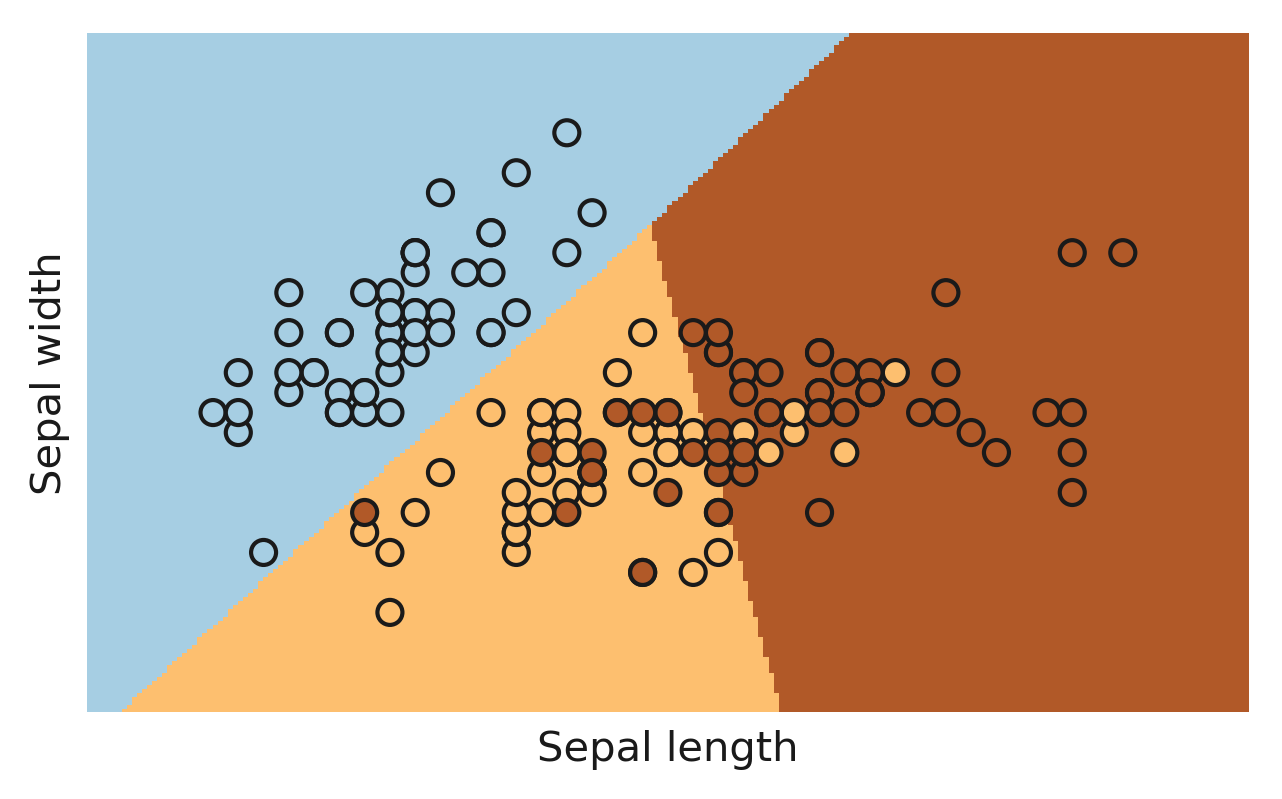
\includegraphics[height=0.33\textwidth]{figures/iris_classification.png} &  
            
\includegraphics[height=0.3\textwidth]{figures/sketches/Large53.jpg}
            \\
            \end{tabular}
            
            \caption[Classification of the iris dataset]{Classification of the iris dataset into three distinct species, based on two features (sepal length and sepal width). Each circle represents a distinct example (i.e. a flower), and its color represents its species. The classifier linearly separates the plane, and the background coloring corresponds to the classifier's prediction for that location in the plane. Circles that are enclosed in a background distinct from them are erroneous predictions.}
            \label{fig:iris_prediction}
        \end{figure}
        
        We can predict the species of a plant (the attribute) based on sepal and petal length and width. This is a classical example, based on the Iris Dataset \cite{fisher1936use}, and represented in figure \ref{fig:iris_prediction}. The classifier is defined as a mapping from any point in the multidimensional space into a vector of probabilities, with a probability for each possible species. An example of plant, with its feature vector, has then an associated most-probable species, that is given as the prediction of the classifier for that data point.
        
        In neuroscience, machine learning has been generally used in conjunction with other statistical techniques to test hypothesis about the underlying attributes in the neural activity. For example: To test whether activity in the visual cortex contains information about a given stimulus, machine learning can be used to predict the stimulus based on the activity \cite{vetter2014decoding}. If predictions are above chance level, then there was information contained in the activity. Moreover, machine learning methods can be used to compare distinct regions, contrasting of their decoding performance and pattern of responses, as exemplified below.
        
        \begin{figure}
            \centering
            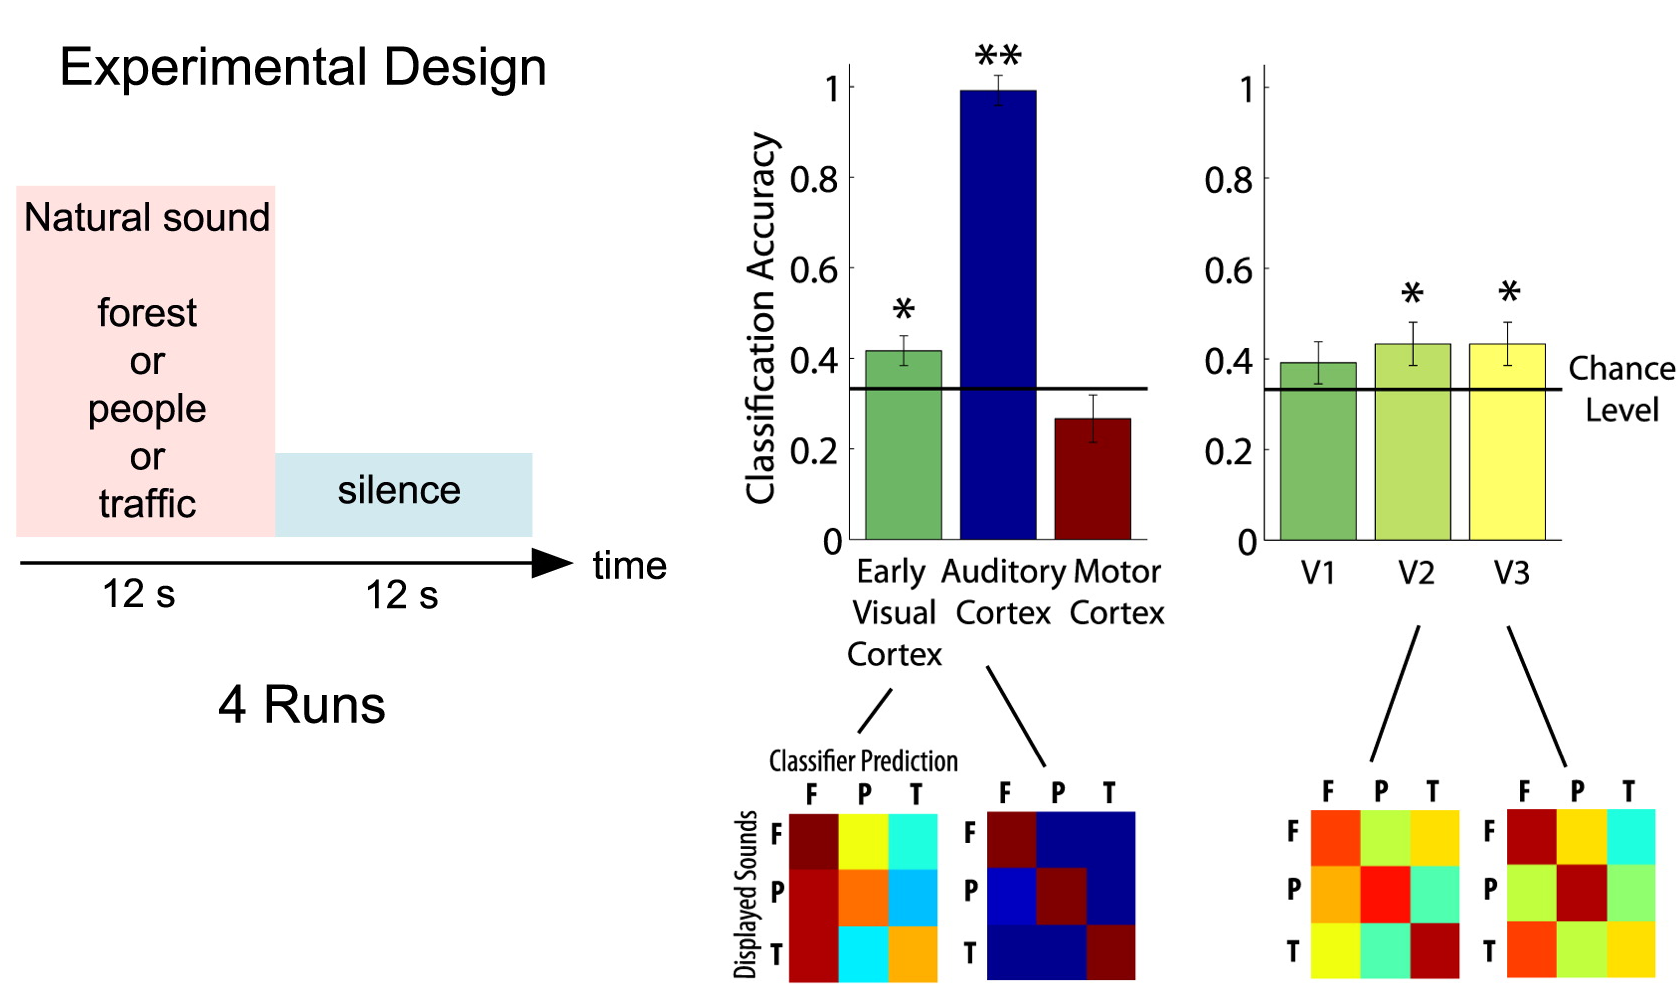
\includegraphics[width=\textwidth]{figures/sketches/sound_prediction_tiny.png}
            \caption[Decoding sound from visual cortex]{Decoding sound from visual cortex. The image shows the design and results for a single experiment using MVPA. A sound is presented, sampled from one of three distinct types of natural sounds, and the subsequent neural activity is fed into a classifier that tries to predict the sound. In the bar plots, the accuracy of classifier predictions is measured for each brain region. Neural activity from three regions is compared, and for three subregions inside the early visual cortex. The heatmaps in the bottom are confusion matrices, that show the count of predictions for each possible combination of displayed sound and predicted sound. Adapted from Vetter et al.~\cite{vetter2014decoding}.}
            \label{fig:prediction_neuro}
        \end{figure}
        
        In figure \ref{fig:prediction_neuro}, Vetter et al. \cite{vetter2014decoding} used machine learning to assess whether multiple regions encoded information about auditory stimuli. After decoding presented sounds (the hidden attribute) from the neural activity of each region, they tested whether the decoding performance was above chance. The predictions were accurate for the auditory cortex, what is not a surprise. A more surprising result was that the early visual cortex also performed above chance. Analyzing more specifically, they showed that this information was mainly on V2 and V3 cortices, and V1 alone did not perform above chance. Vetter et al. presented four other experiments and results to demonstrate that the brain can translate abstract information to encode in the early visual cortex \cite{vetter2014decoding}.
        
        One advantage of machine learning techniques is their generality: they make less assumptions than classical analysis. Supervised learning, the kind most used in MVPA, encompasses two main techniques: Regression and Classification. They both tackle the same problem of decoding hidden attributes, but make different assumptions about the encoding. In regression the attribute is considered continuous, while in classification the attribute is one of a set. In both cases, there are many degrees of freedom that are fitted from the data, lessening the need for domain knowledge about the encoding\footnote{In the machine learning community, domain knowledge about the encoding is usually referred as \textit{feature engineering}.}.

        % \cite{merchant2008we} % MVPA temporal generalization

\section{Representation}
\label{sec:representation}
    The notion that representation is central to cognition is old \cite[p.~134-140]{rosch1991embodied} and it grounds one central method for assessing brain function: the search for neural correlates of measurable quantities. We know that there are neurons in the primary visual cortex that represent (i.e., encode) inclination angles of bars \cite[p.~13]{dayan2001theoretical} and neurons in the primary motor cortex that represent the angle of reaching movements \cite[p.~14]{dayan2001theoretical}. But more complex concepts -- like one's grandmother \cite{gross2002genealogy} or causality \cite{blakemore2001brain} -- may be highly dependant on the context to be captured with such specific correlates.
    
    Since the early days of neuroscience, there is a debate about the general form of brain representation. Cognitivists posed that representation is formed by well defined strings of symbols that logically interact, while connectionists maintained that representation is distributed in the neuronal connections. The former vision is exemplified in the seminal McCulloch \& Pitts paper \cite{mcculloch1943logical}, where they propose that "To each reaction of any neuron there is a corresponding assertion of a simple proposition". The latter is commonly exemplified by modern machine learning \textit{neural networks}, where single neurons rarely have some \textit{meaning} on their own. Connectionism gained strength in the late 80's by the seminal Parallel Distributed Processing \cite{mcclelland1986parallel}, and although many of its related algorithms fall short of biological plausibility, there are those such as Hopfield Networks and Boltzmann Machines, based on autoassociative rules reminiscent of Hebbian learning, that made their way into modern models of brain function \cite{mceliece1987capacity}. 

    The debate between Cognitivism and Connectionism cuts across levels of analysis, making it specially intricate. Implementational connectionists pose that the views are consistent with one another, with the brain's neural network acting as a distributed system that, when analyzed through a higher level of abstraction, is a symbolic processor \cite{bechtel1988connectionism}. Alongside this theoretical studies, measurements of neural activity are generally studied through the lens of representation, with the most prominent being single neuron representations \cite{quiroga2005invariant}, mainly consistent with the Cognitivist view.

    Single neuron representations have been specially studied by the vision community \cite{deyoe1988concurrent, bell1997independent, ito2004representation, lee2008sparse}, but recent contributions have taken this approach much beyond the sensory realm, to the more abstract domains of \textit{space} and \textit{time} \cite{eichenbaum2014time}. \textit{Place cells} are neurons that fire in specific locations of some environment \cite{foster2006reverse}, and are mainly present in the Hippocampus \cite{o1979review}. In the same way, \textit{time cells} fire in specific times after some event \cite{tiganj2016sequential, eichenbaum2014time}, and may serve as temporal basis for representations of the world \cite{ludvig2008stimulus}, being complemented by \textit{ramping neurons}, that linearly increase or decrease their activity during a time interval \cite{morrison2009convergence, kim2013neural, tiganj2016sequential, parker2016timing}.

    %, bestowing the brain with a whole new dimension along which to relate its activity \cite{eichenbaum2014time}

    It becomes clear, through the previous paragraphs, that the search for neural correlates deeply entangles the representational and implementational levels, and may be better understood through some conceptual distancing. Representations have to do with the internal objects that are transformed through some algorithm, for which many implementations are possible. Take the following example: time is a quantity that evolves monotonically and linearly, and so does its representation. The monotonicity can be achieved by any phase-space trajectory, with the condition that it does not cross itself. In addition, linearity can be achieved by a simple nonlinear regression reading-out the monotonic activity. The regression could be implemented having another general trajectory as output \cite{gallant1975nonlinear} or a single ramping neuron: The choice of input and output is by no means obvious, and depend at least as much in the computational goals as the implementational constrains.
    
    Although there are many examples of quantities encoded in single neurons, such as aforementioned, it is not necessary that particular neurons have such interpretable roles. Phase space trajectories can be composed by the activity of populations \cite{shamir2014emerging, quiroga2009extracting}, as well as less explicit dimensions such as post-synaptic sensitivity \cite{motanis2018short}, and neuromodulation effects \cite{friston2009free, friston2010free}. While the latter two also affect behavior \cite{wolff2017dynamic}, we do not account for them in the present work, as they are not directly detectable from neural activity. Hence, the present work focuses in population activity.
    % accumulators bueti2011physiological, wittmann2010accumulation
    
    Population codes have the capacity to carry much more information than single neuron codes \cite{hardy2016neurocomputational}, but since population patterns are by definition multivariate, their study requires more elaborate techniques \cite{quiroga2009extracting}, such as Machine Learning. 
    There are many ways in which a given neural population may encode information \cite{quiroga2009extracting, shamir2014emerging, mello2015scalable}, and we discuss some proposals specific for time in the next chapter.